% Preamble

\documentclass[../main.tex]{subfiles}
\graphicspath{{\subfix{../images/}}}

\begin{document}



\section{Introduction}

Transmitted data through networks has increassed in last decade. Networks, originally focused on voice, now are moving to multimedia and interactive services, resulting in a set of new requirements:

\begin{itemize}
	\item Efficient use of bandwidth, which is highly demanded.
	\item Flexibility for changing services and usage.
	\item Achievement of coverage for all digital service, also known as ``one network for everything'' (B-ISDN).
\end{itemize}

For that purpose, there have been developed flexible network architectures for access and transport:

\begin{itemize}
	\item Integrated Services Digital Network (ISDN).
	\item Digital Subscriber Line (DSL).
	\item Synchronous Digital Hierarchy (SDH) / Synchronous Optical NETwork (SONET).
	\item Dense Wavelength Division Multiplexing ((D)WDM).
	\item Asynchronous Transfer Mode (ATM).
	\item {
		Wireless systems:
		\begin{itemize}
			\item Multichannel Multipoint Distribution Service (MMDS).
			\item Local Multipoint Distribution Service (LMDS).
			\item Wireless Local Area Networks (WLAN).
			\item Worldwide Interoperability for Microwave Access (WiMAX).
		\end{itemize}
	}
\end{itemize}

Those architectures can be classified in two kinds of complementary networks:

\begin{itemize}
	\item Access Networks: They allow the service operator to give users the access to services, this is, they are managed and perform terminal communications activities. Some examples are ISDN, PSTN, xDSL and WiFi.
	\item Core Networks (also called Transport Networks): High capacity networks to interconnect other networks such as the access networks, this is, they are unmanaged and perform intermediate communications activities. Some examples are SDH, ATM, (D)WDM and IP.
\end{itemize}

The implementation of these systems still must face some limitations:

\begin{itemize}
	\item Congestion due to bandwidth limitation.
	\item Adaptation to new users requirements, like data type (video, multimedia, etc.) and service (P2P, instantaneous digital communicarion, etc.).
\end{itemize}

Previous to current technology, Plesiochronous Digital Hierarchy (PDH) was a standard with the following specifications:

\begin{itemize}
	\item Time Division Multiplexing (TDM).
	\item European PDH: 30 channel (E1) at $64 kbps$ (E0). Hierarchy up to E4.
	\item American PDH: 24 channels (T1) at $64 kbps$ (T0) (two of them at $56 kbps$).
\end{itemize}

In optical networks, the maximum length of a section (span) can be obtained with:

$$
	L = \frac {104 000} {CD \cdot R_{b}^2} [km]
$$

Where:

\begin{itemize}
	\item $CD$: Chromatic dispersion in \textbf{ps}.
	\item $R_b$: Bit rate in \textbf{Gbps}.
\end{itemize}

\iffalse

\subsection{Optical networks}

AAAA

\fi

\section{Integrated Services Digital Network (ISDN)}

\subsection{Introduction}

ISDN provides the standards for a network that is able to carry different types of information (voice, data, texts, images, ...) in digital format and end to end. It is an evolution from telephony Integrated Digital Network (IDN), so it offers connections up to $64 kbps$ by circuit switching and also packet switching services are allowed. It provides an integrated subscriber access. Its evolution comprises:

\begin{itemize}
	\item {
		N-ISDN:
		\begin{itemize}
			\item Connection up to $64 kbps$.
			\item Connection up to $n \times 64 kbps$ ($< 2 Mbps$).
		\end{itemize}
	}
	\item B-ISDN: Connections above $2 Mbps$.
\end{itemize}

\subsection{Reference configuration}

ISDN's goal is to use a reduced set of interfaces between user and network for low cost and to hold a large number of applications, equipments and configurations. Terminals are:

\begin{itemize}
	\item R: It connects terminal equipment with terminal adapters: TE - TA.
	\item S: It connects terminal equipment with network terminations and terminal adapters with network terminations: TE - NT, TA - NT.
	\item T: It connects terminal equipment with network terminations, terminal adapters with network terminations and network terminations with other network terminations: TE - NT, TA - NT, NT - NT.
	\item U: It connects network terminations with line terminations: NT - LT.
	\item V: It connects line terminations with exchange terminations: LT - ET.
\end{itemize}

\begin{figure}[H]
	\centering
	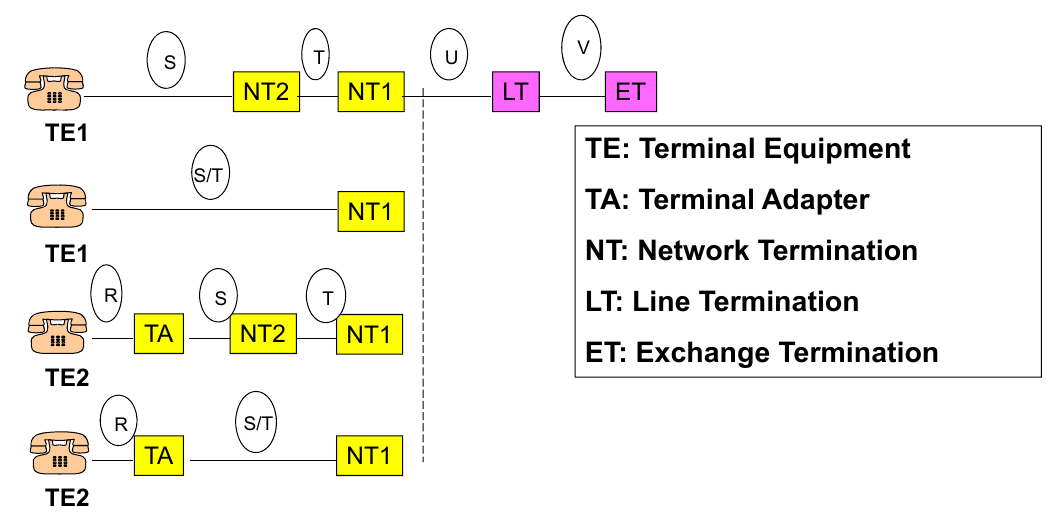
\includegraphics[
		width=12cm,
		%height=15cm
	]{images/Tema 3/Reference configuration.png}
	\caption{
		\label{fig:unit3_ref_conf}
		ISDN reference configuration
	}
\end{figure}

\begin{table}[H]
	\centering
	\begin{tabular}{|c|c|c|c|c|c|}
		\hline
		   & TE & TA & NT & LT & ET \\
		\hline
		TE & & R & S, T & & \\
		\hline
		TA & \cellcolor{black} & & S, T & & \\
		\hline
		NT & \cellcolor{black} & \cellcolor{black} & T & U & \\
		\hline
		LT & \cellcolor{black} & \cellcolor{black} & \cellcolor{black} & & V \\
		\hline
		ET & \cellcolor{black} & \cellcolor{black} & \cellcolor{black} & \cellcolor{black} & \\
		\hline
	\end{tabular}
	\caption{
		\label{tab:isdn_ref_conf}
		ISDN reference configuration
	}
\end{table}

\subsection{Channels}

ISDN establishes different types of data channel whose implementation is done at bit level, inside data frames. There are three types:

\begin{itemize}
	\item Channel B: Used to transport data (including voice). Its data rate is 64 kbps.
	\item Channel D: Used for signaling (low data rate). Its data rate can be 16 kbps or 64 kbps.
	\item {
		Channel H: Used to transport data. Its data rate is higher than 64 kbps. The are three types:
		\begin{itemize}
			\item H0: Its data rate can be 384 kbps or 375 kbps (6 channels B).
			\item H11: Its data rate can be 1536 kbps or 1500 kbps (24 channels B). It is used in countries with DS1 (1544 kbps) hierarchy.
			\item H12: Its data rate can be 1920 kbps or 1875 kbps (30 channels B). It is used in countries with E1 (2048 kbps) hierarchy.
		\end{itemize}
	}
\end{itemize}

\subsection{Transmission}

For transmission, we use several channels multiplexed in TDM (frame). For each purpose:

\begin{itemize}
	\item Voice transmission and 3.1 kHz digital audio. 8 bits each, 125 $\mu$s (64 kbps).
	\item Data transmission. Several data rates adapted to 64 kbps.
	\item {
		Signaling:
		\begin{itemize}
			\item Data rate up to 16 kbps or 64 kbps.
			\item It is fixed in the frame, but it can be used for data in certain cases.
		\end{itemize}
	}
\end{itemize}

\subsection{Access type}

There are two access types, basic rate and primary rate, which will be able to work in specific interfaces.

\begin{table}[H]
	\centering
	\begin{tabular}{|c|c|c|c|c|c|}
		\hline
		& R & S & T & U & V \\
		\hline
		Basic rate & & X & & X & \\
		\hline
		Primary rate & & & & X & \\
		\hline
	\end{tabular}
	\caption{
		\label{tab:isdn_interfaces_rates}
		ISDN interface rates
	}
\end{table}

\subsubsection{Basic rate}

The useful data rate is calculated in the following way:

$$
	2B + D = 2 \times 64 kbps + 16 kbps = 144 kbps
$$

It can be supported by almost all current at 2W by using duplex digital multiplex transmission (echoes cancellation). The main application is residential or small offices with few terminals. We distinguish two types depending on the interface:

\begin{itemize}
	\item {
		At S interface:
		\begin{itemize}
			\item The data rate is 192 kbps.
			\item {
				The frame:
				\begin{itemize}
					\item Frames have 48 bits ($L = 48 [b] $) and they are transmitted in 250 microseconds ($T_{tx} = 250 [\mu s/frame]$), resulting in 4000 frames per second ($f_{tx} = 1/T_{tx} = 4000 [frames/s]$) or 192 kbps ($C = f_{tx} \cdot L = 192 [kbps]$).
					\item Each channel B is divided in two groups of slots, B1 and B2.
					\item Each channel B group is composed by two 8-bit slots, resulting in four 8-bit slots.
					\item The channel B slots sent alternatively and between each channel B slot one channel D slot (1 bit) is inserted, resulting in 36 bits.
					\item Only 36 useful bits of 48.
					\item {
						One single channel B group rate:

						$
							\frac {2 \cdot 8 [b]} {250 \cdot 10^{-6} [s]} = 64 \cdot 10^3 [bps]
						$
					}
					\item {
						B channel rate:

						$
							\frac {4 \cdot 8 [b]} {250 \cdot 10^{-6} [s]} = 128 \cdot 10^3 [bps]
						$
					}
					\item {
						D channel rate:

						$
							\frac {4 \cdot 1 [b]} {250 \cdot 10^{-6} [s]} = 16 \cdot 10^3 [bps]
						$
					}
					\item {
						Total rate:

						$
							\frac {4 \cdot 8 [b] + 4 \cdot 1 [b]} {250 \cdot 10^{-6} [s]} = 144 \cdot 10^3 [bps]
						$
					}
				\end{itemize}

				\begin{figure}[H]
					\centering
					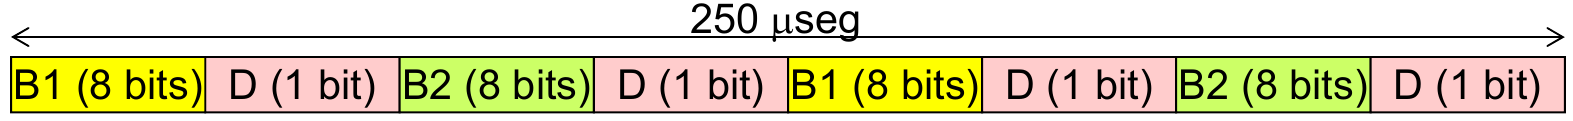
\includegraphics[
						width=10cm,
						%height=15cm
					]{images/Tema 3/Frame in S interface at basic rate.png}
					\caption{
						\label{fig:unit3_frame_S_basic}
						Frame in S interface at basic rate
					}
				\end{figure}
			}
			\item {
				Line coding:
				\begin{itemize}
					\item {
						Alternate Mark Inversion (AMI) is used:
						\begin{itemize}
							\item 0 $\rightarrow$ No signal.
							\item 1 $\rightarrow$ RZ bipolar pulses alternating the sign.
						\end{itemize}
					}
					\item {
						Frame alignment is obtained by violating the 1s signs' alternation.

						\begin{figure}[H]
							\centering
							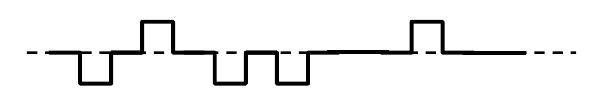
\includegraphics[
								width=10cm,
								%height=15cm
							]{images/Tema 3/Line coding in interface S at basic rate.png}
							\caption{
								\label{fig:unit3_coding_S_basic}
								Line coding in interface S at basic rate (1s signs' alternation)
							}
						\end{figure}
					}
					\item {
						The NT power supplies the terminal:
						\begin{itemize}
							\item Superimposing the DC signal into the signal or in a different pair.
							\item In a power failure, it gets the 48 V from the local exchange and it can power only one terminal (telephone).
						\end{itemize}
					}
				\end{itemize}
			}
		\end{itemize}
	}
	\item {
		At U interface:
		\begin{itemize}
			\item The data rate is 160 kbps.
			\item {
				Frame:
				\begin{itemize}
					\item {
						Each frame (240 bits) has 12 sets of 2B+D (18 bits) jointly with maintenance (6 bits) and synchronism (18 bits).

						\begin{figure}[H]
							\centering
							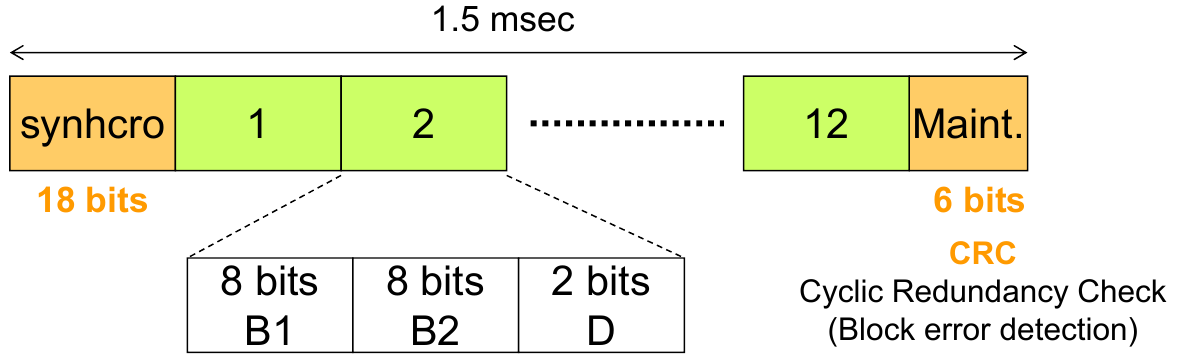
\includegraphics[
								width=12cm,
								%height=15cm
							]{images/Tema 3/Frame in U interface at basic rate.png}
							\caption{
								\label{fig:unit3_frame_U_basic}
								Frame in U interface at basic rate
							}
						\end{figure}
					}
					\item $80000 [pulses/sec]$ are sent in 2B1Q ($240[b]/1.5[ms] = 160 [kbps]$).
					\item {
						Synchronism slot rate:

						$
							\frac {1 \cdot 18 [b]} {1.5 \cdot 10^{-3} [s]} = 12 \cdot 10^3 [bps]
						$
					}
					\item {
						Maintenance slot rate:

						$
							\frac {6 [b]} {1.5 \cdot 10^{-3} [s]} = 4 \cdot 10^3 [bps]
						$
					}
					\item {
						One single channel B group rate:

						$
							\frac {12 \cdot 8 [b]} {1.5 \cdot 10^{-3} [s]} = 64 \cdot 10^3 [bps]
						$
					}
					\item {
						B channel rate:

						$
							\frac {12 \cdot 2 \cdot 8 [b]} {1.5 \cdot 10^{-3} [s]} = 128 \cdot 10^3 [bps]
						$
					}
					\item {
						D channel rate:

						$
							\frac {12 \cdot 2 [b]} {1.5 \cdot 10^{-3} [s]} = 16 \cdot 10^3 [bps]
						$
					}
					\item {
						Total channels rate:

						$
							\frac {12 \cdot 2 \cdot 8 [b] + 12 \cdot 2 [b]} {1.5 \cdot 10^{-3} [s]} = 144 \cdot 10^3 [bps]
						$
					}
					\item {
						Total rate:

						$
							\frac {1 \cdot 18 [b] + 1 \cdot 6 [b] + 12 \cdot 2 \cdot 8 [b] + 12 \cdot 2 [b]} {1.5 \cdot 10^{-3} [s]} = 160 \cdot 10^3 [bps]
						$
					}
				\end{itemize}
			}
			\item {
				Line coding for reducing the symbol rate:
				\begin{itemize}
					\item {
						2B1Q (ANSI standard and the trend is to keep it alone). Two bits are transmitted by a quaternary pulse ($-3$, $-1$, $+1$, $+3$).

						\begin{figure}[H]
							\centering
							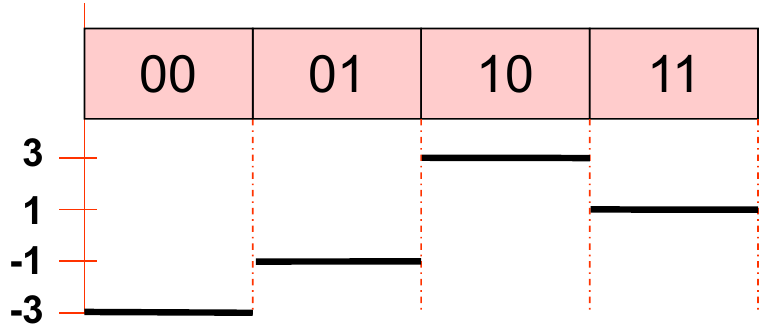
\includegraphics[
								width=6cm,
								%height=15cm
							]{images/Tema 3/2B1Q.png}
							\caption{
								\label{fig:unit3_2B1Q}
								2B1Q coding
							}
						\end{figure}
					}
					\item 4B3T
				\end{itemize}
			}
		\end{itemize}
	}
\end{itemize}

\subsubsection{Primary rate}

The useful data rate is calcluated in the following way for Europe:

$$
	30B + D = 30 \times 64 [kbps] + 64 [kbps] = 1984 [kbps]
$$

And for USA:

$$
	23B + D = 23 \times 64 [kbps] + 64 [kbps] = 1536 [kbps]
$$

Global data rate, including synchronism method, is 2048 kbps (PCM). Its applications are those that require both low capacity and high capacity user exchanges. Other configurations can be supported ($5H0 + D$, $H12 + D$, $31B$). It always work at 4W. It works in U interface:

\begin{itemize}
	\item {
		Line coding:
		\begin{itemize}
			\item The code method is High Density Bipolar Code (HDB3). It is similar to AMI, but limiting the transmission of many zeros in a row.
			\item In HDB3, any instance of four consecutive 0 bits is replaced with one of the patterns $000V$ (odd) or $B00V$ (even). The choice is made to ensure that consecutive violations $V$ are of differing polarity, this is, separated by an odd number of normal $+$ or $-$ marks.
			\item {
				To determine which pattern to use, one must count the number of pluses ($+$) and the number of minuses ($-$) (equivalently, the number of ones) since the last violation bit V:
				\begin{itemize}
					\item If the result is an odd number then $000-$ or $000+$ ($000V$) is used.
					\item If the result is an even number then $+00+$ or $-00-$ ($B00V$) is used.
				\end{itemize}
			}
			\item {
				To determine which polarity to use, one must look at the pulse preceding the four zeros:
				\begin{itemize}
					\item If odd ($000V$) form must be used, then $V$ simply copies the polarity of last pulse. Then, we can identify this sequence with the shape: $\ldots X000X \ldots$
					\item If even ($B00V$) form must be used, then $B$ and $V$ chosen will have the opposite polarity of the last pulse. Then, we can identify this sequence with the shape: $\ldots YX00X \ldots$
				\end{itemize}
			}
		\end{itemize}
		\begin{table}[H]
			\centering
			\begin{tabular}{|l|c|c|c|}
				\hline
				Parity of $+/-$ bits since previous $V$	& Pattern					& Previous pulse	& Code \\
				\hline
				\multirow{2}{*}{Even}					& \multirow{2}{*}{$B00V$}	& $+$				& $-00-$ \\
				\cline{3-4}
														&							& $-$				& $+00+$ \\
				\hline
				\multirow{2}{*}{Odd}					& \multirow{2}{*}{$000V$}	& $+$				& $000+$ \\
				\cline{3-4}
														&							& $-$				& $000-$ \\
				\hline
			\end{tabular}
			\caption{
				\label{tab:HDB3}
				High Density Bipolar Code (HDB3)
			}
		\end{table}
	}
	\item {
		Frame in Europe:

		\begin{itemize}
			\item {
				256 bits ($L = 256 [b/frame]$) in 125 microseconds ($T_{tx} = 125 [\mu s]$), 8000 frames per second ($f_{tx} = 1/T_{tx} = 8000 [frames/s]$), resulting in a 2048 kbps data rate ($C = f_{tx} \cdot L = 2048 [kbps]$).

				\begin{figure}[H]
					\centering
					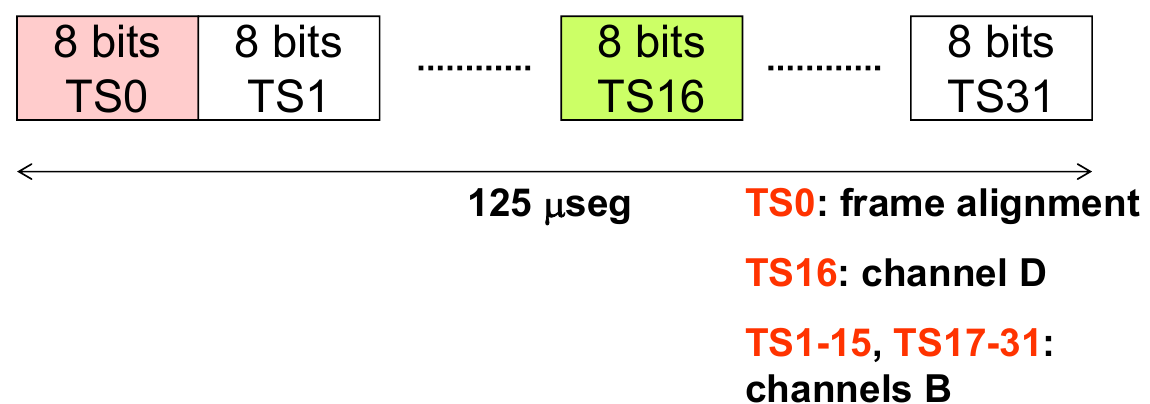
\includegraphics[
						width=9cm,
						%height=15cm
					]{images/Tema 3/Frame in U interface at primary rate (Europe).png}
					\caption{
						\label{fig:unit3_frame_U_primary_EU}
						Frame in U interface at primary rate (Europe)
					}
				\end{figure}
			}
			\item {
				Alignment slot rate:

				$
					\frac {1 \cdot 8 [b]} {125 \cdot 10^{-6} [s]} = 64 \cdot 10^3 [bps]
				$
			}
			\item {
				One single B channel slot rate:

				$
					\frac {1 \cdot 8 [b]} {125 \cdot 10^{-6} [s]} = 64 \cdot 10^3 [bps]
				$
			}
			\item {
				B channel rate:

				$
					\frac {30 \cdot 8 [b]} {125 \cdot 10^{-6} [s]} = 1920 \cdot 10^3 [bps]
				$
			}
			\item {
				D channel rate:

				$
					\frac {1 \cdot 8 [b]} {125 \cdot 10^{-6} [s]} = 64 \cdot 10^3 [bps]
				$
			}
			\item {
				Total channels rate:

				$
					\frac {30 \cdot 8 [b] + 1 \cdot 8 [b]} {125 \cdot 10^{-6} [s]} = 1984 \cdot 10^3 [bps]
				$
			}
			\item {
				Total rate:

				$
					\frac {1 \cdot 8 [b] + 30 \cdot 8 [b] + 1 \cdot 8 [b]} {125 \cdot 10^{-6} [s]} = 2048 \cdot 10^3 [bps]
				$
			}
		\end{itemize}
	}
	\item {
		Frame in USA:

		\begin{itemize}
			\item {
				193 bits ($L = 193 [b/frame]$) in 125 microseconds ($T_{tx} = 125 [\mu s]$), 8000 frames per second ($f_{tx} = 1/T_{tx} = 8000 [frames/s]$), resulting in a 1544 kbps data rate ($C = f_{tx} \cdot L = 1544 [kbps]$).

				\begin{figure}[H]
					\centering
					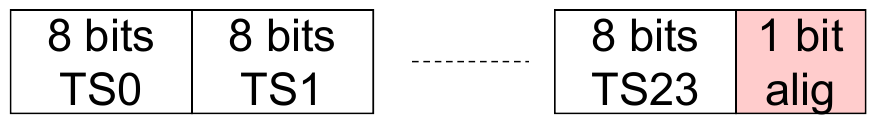
\includegraphics[
						width=7cm,
						%height=15cm
					]{images/Tema 3/Frame in U interface at primary rate (USA).png}
					\caption{
						\label{fig:unit3_frame_U_primary_USA}
						Frame in U interface at primary rate (USA)
					}
				\end{figure}
			}
			\item {
				Alignment slot rate:

				$
					\frac {1 \cdot 1 [b]} {125 \cdot 10^{-6} [s]} = 8 \cdot 10^3 [bps]
				$
			}
			\item {
				One single B channel slot rate:

				$
					\frac {1 \cdot 8 [b]} {125 \cdot 10^{-6} [s]} = 64 \cdot 10^3 [bps]
				$
			}
			\item {
				B channel rate:

				$
					\frac {23 \cdot 8 [b]} {125 \cdot 10^{-6} [s]} = 1472 \cdot 10^3 [bps]
				$
			}
			\item {
				D channel rate:

				$
					\frac {1 \cdot 8 [b]} {125 \cdot 10^{-6} [s]} = 64 \cdot 10^3 [bps]
				$
			}
			\item {
				Total channels rate:

				$
					\frac {23 \cdot 8 [b] + 1 \cdot 8 [b]} {125 \cdot 10^{-6} [s]} = 1536 \cdot 10^3 [bps]
				$
			}
			\item {
				Total rate:

				$
					\frac {23 \cdot 8 [b] + 1 \cdot 8 [b] + 1 \cdot 1 [b]} {125 \cdot 10^{-6} [s]} = 1544 \cdot 10^3 [bps]
				$
			}
		\end{itemize}
	}
\end{itemize}

\section{Digital Subscriber Loop (xDSL)}

\subsection{Introduction}

Copper subscriber loops are highly deployed. They have been used to increased data rate transmission, first, with modems, up to 56 kbps, later, on ISDN, up to 128 kbps. There are new technologies for increasing data rate over Mbps, all of them named Digital Subscriber Loop (xDSL):

\begin{itemize}
	\item High data rate DSL (HDSL): 2 Mbps duplex.
	\item Asymmetric DSL (ADSL): 1-8 Mbps DS or 16-640 Kbps US.
	\item Very high data rate DSL (VDSL): 13-52 Mbps DS or 1.5-2.3 Mbps US.
\end{itemize}

There are several systems for each technology: ADSL, ADSL2, ADSL2+, VDSL, VDSL2,... Mainly multi-carrier modulation. Echoe’s cancellation might be needed.

\subsection{Asymmetric DSL (ADSL)}

Different data rates for different directions (User $\leftrightarrow$ Network). Thus, different modems: ATU-R and ATU-C. There is a splitter system, two filters separate telephony from ADSL.

\begin{figure}[H]
	\centering
	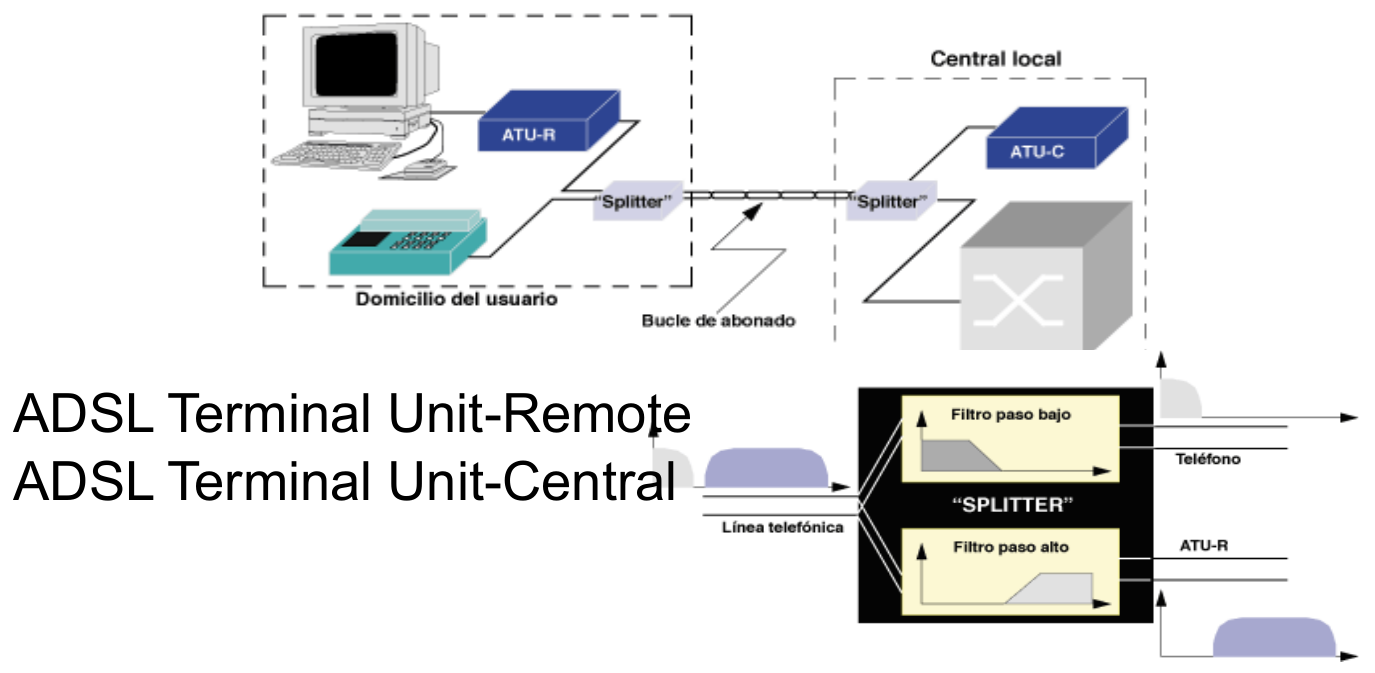
\includegraphics[
		width=14cm,
		%height=15cm
	]{images/Tema 3/ADSL.png}
	\caption{
		\label{fig:unit3_ADSL_scheme}
		ADSL scheme
	}
\end{figure}

It uses DMT modulation:

\begin{itemize}
	\item {
		Spectrum:

		\begin{figure}[H]
			\centering
			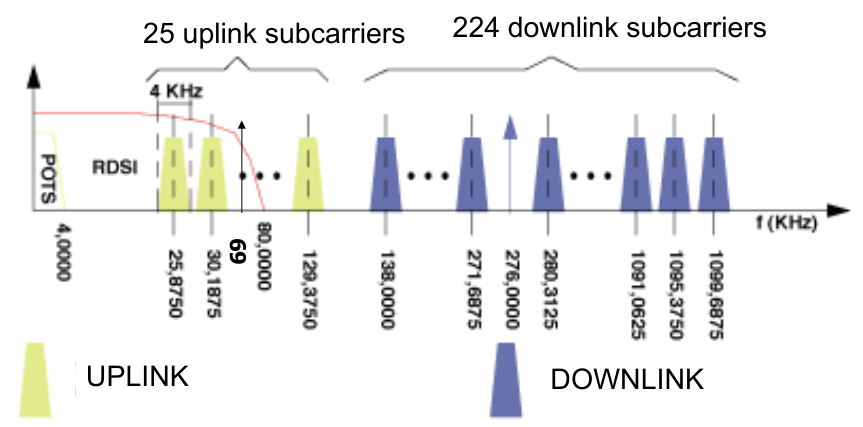
\includegraphics[
				width=10cm,
				%height=15cm
			]{images/Tema 3/ADSL spectrum.png}
			\caption{
				\label{fig:unit3_ADSL_spectrum}
				ADSL spectrum
			}
		\end{figure}
	}
	\item {
		Echo cancellation:

		\begin{figure}[H]
			\centering
			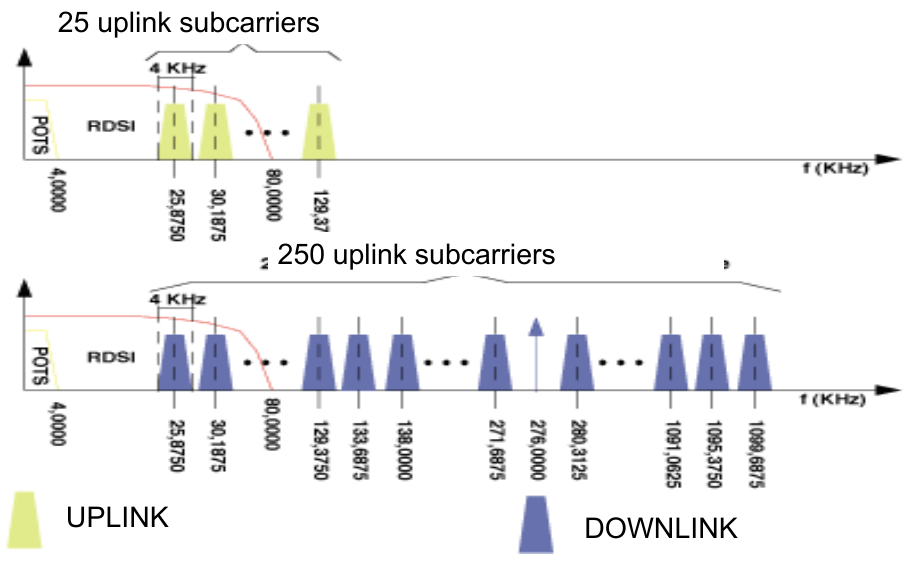
\includegraphics[
				width=10cm,
				%height=15cm
			]{images/Tema 3/ADSL echo cancellation.png}
			\caption{
				\label{fig:unit3_ADSL_echo}
				ADSL echo cancellation
			}
		\end{figure}
	}
\end{itemize}

Here is a comparison:

\begin{figure}[H]
	\centering
	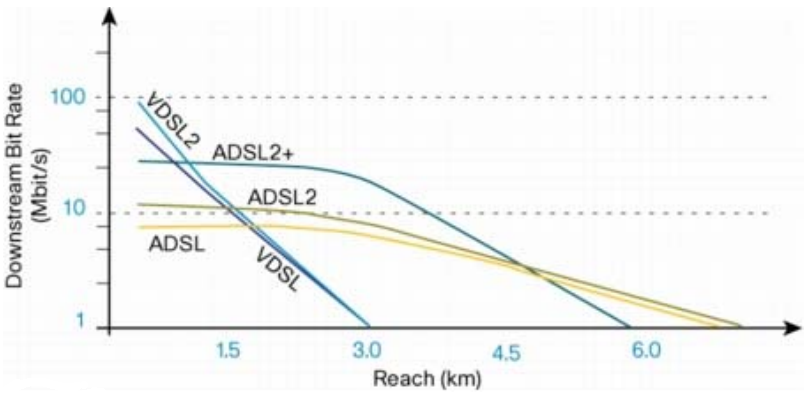
\includegraphics[
		width=12cm,
		%height=15cm
	]{images/Tema 3/ADSL comparison.png}
	\caption{
		\label{fig:unit3_ADSL_comparison}
		ADSL comparison
	}
\end{figure}

\section{Synchronous Digital Hierarchy (SDH)}

\subsection{Introduction}

The SDH is a hierarchical set of digital transport structures, standardized for the transport of suitably adapted payloads over physical transmission networks. ITU-T provides with a set of recommendations: G.707, G.772, G.774.x, G.780, G.783, G.784, G.803, G.810, G.811, G.813, G.825, ...

The initial objectives were modest, such as the connection of different manufactures’ optical equipments (transversal compatibility). It is indeed a multiplexing technique the one that allows the transportation of ``payloads'' from digital hierarchies (1.5 Mbps in USA and Japan, 2 Mbps at international level). Motivations behind SDH include:

\begin{itemize}
	\item High speed optical elements.
	\item Reduction in wires.
	\item Remote managements of equipments and circuits.
	\item Transversal compatibility.
	\item Broadband and narrowband compatibility.
\end{itemize}

\begin{figure}[H]
	\centering
	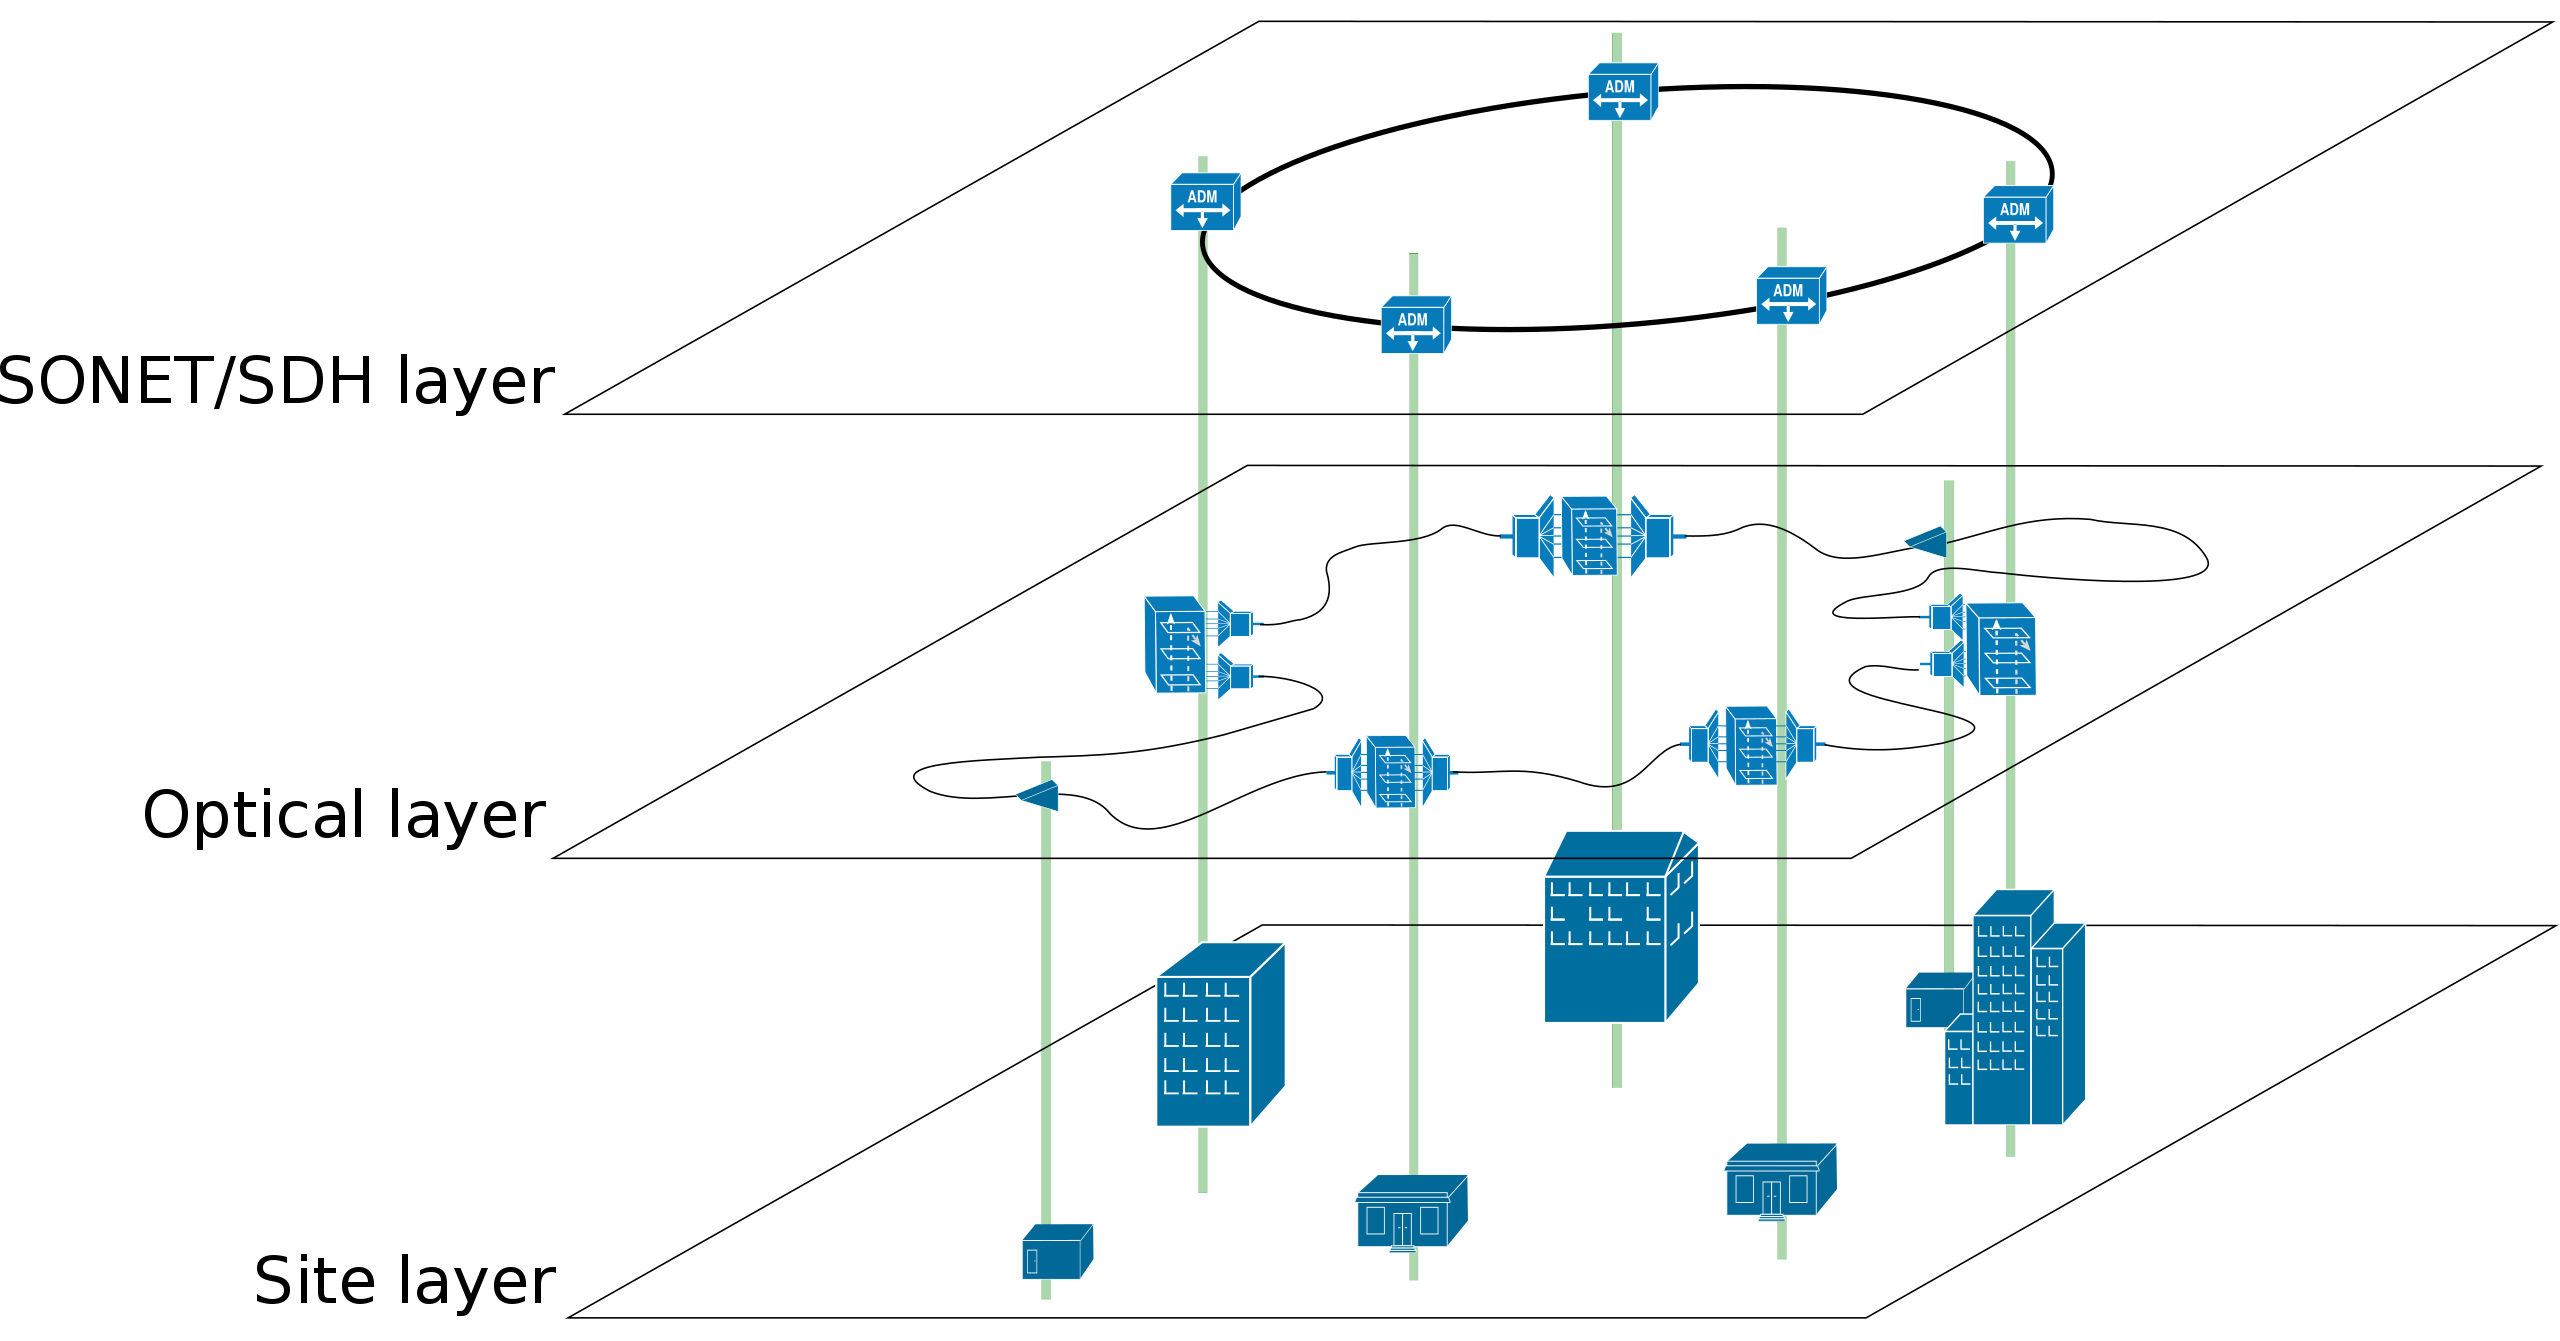
\includegraphics[
		width=15cm,
		%height=15cm
	]{images/Tema 3/Network_Overlay.png}
	\caption{
		\label{fig:unit3_SDH_ring_arch}
		Transport network based on SONET/SDH ring architecture.
	}
\end{figure}

\subsection{Synchronous Transfer Module (STM-N)}

SDH defines a format for transfer among network called Synchronous Transfer Module (STM), which is defined for different levels (N).

\subsubsection{Levels}

\begin{tabular}{|c|c|c|c|}
	\hline
	STM-N	& Digital hierarchy	& Rate (Mbps)	& Electrical/Optical interface \\
	\hline
	SMT-1	& Level 1			& 155,520		& G.703/G.957 \\
	\hline
	STM-4	& Level 4			& 622,020		& ---/G.957 \\
	\hline
	STM-16	& Level 16			& 2488,320		& ---/G.957 \\
	\hline
	STM-64	& Level 64			& 9953,280		& ---/G.957 \\
	\hline
	STM-256	& Level 256			& 9953,280		& ---/G.957 \\
	\hline
\end{tabular}

\subsubsection{STM-1 frame structure}

STM-1 frame structure can be described with the following points:

\begin{itemize}
	\item $9 [rows] \times 270 [columns]$
	\item Each cell is an octet (a byte $B$).
	\item Capacity: $9 \times 270 [B] = 2430 [B] = 19440 [b]$
	\item Frame length: $125 [\mu s] \rightarrow T_{tx} = 125 [\mu s]$
	\item Section OverHead: $SOH = RSOH (3 \times 8 [B] = 24 [B]) + MSOH (5 \times 8 [B] = 40 [B]) = 64 [B]$
	\item Pointer: $1 \times 8 [B] = 8 [B]$
	\item Payload: $9 \times 262 [B] = 2358 [B]$
	\item $R_b = 8000 [frame/s] \cdot 2430 [B/frame] \cdot 8 [b/B] = 155520000 [bps]$
\end{itemize}

\begin{figure}[H]
	\centering
	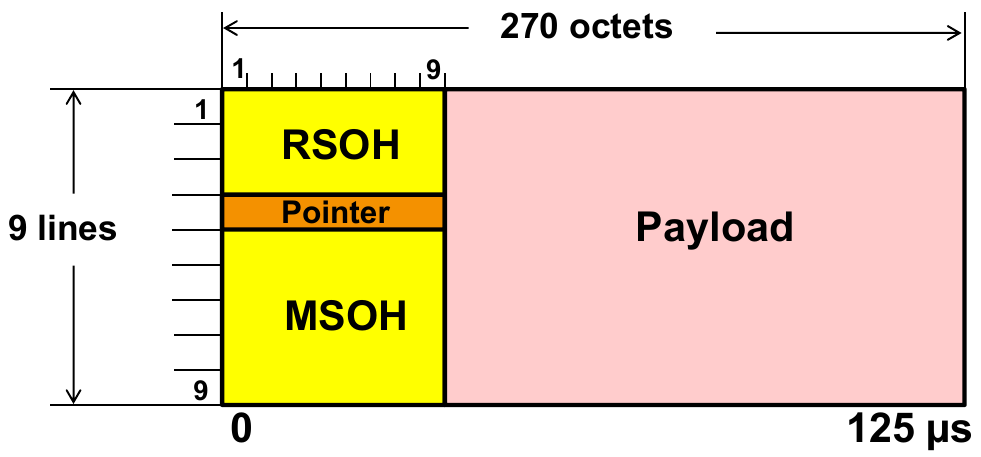
\includegraphics[
		width=10cm,
		%height=15cm
	]{images/Tema 3/STM-1 frame.png}
	\caption{
		\label{fig:unit3_STM1_frame}
		STM-1 frame
	}
\end{figure}

\subsubsection{Inserting C4 into STM-1}

To manage payload, a virtual container must be inserted:

\begin{itemize}
	\item C-x (Container): Spatial division (time too) for the payload.
	\item VC-x (Virtual Container)
	\item AU-x (Administrative Unit): spatial division for the frame into the line
	\item AU-PTR: pointer, indicates the starting point of a VC-x within the STM-1
\end{itemize}

\begin{figure}[H]
	\centering
	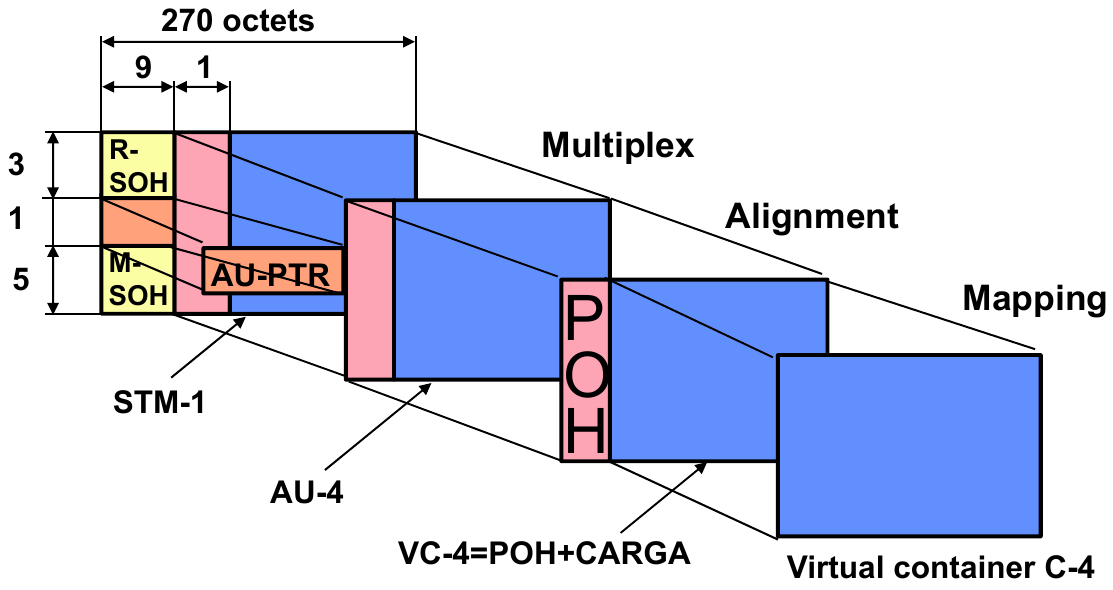
\includegraphics[
		width=10cm,
		%height=15cm
	]{images/Tema 3/STM-1 frame with C4.png}
	\caption{
		\label{fig:unit3_STM1_C4}
		STM-1 frame with C4
	}
\end{figure}

\subsection{Multiplex}

\begin{figure}[H]
	\centering
	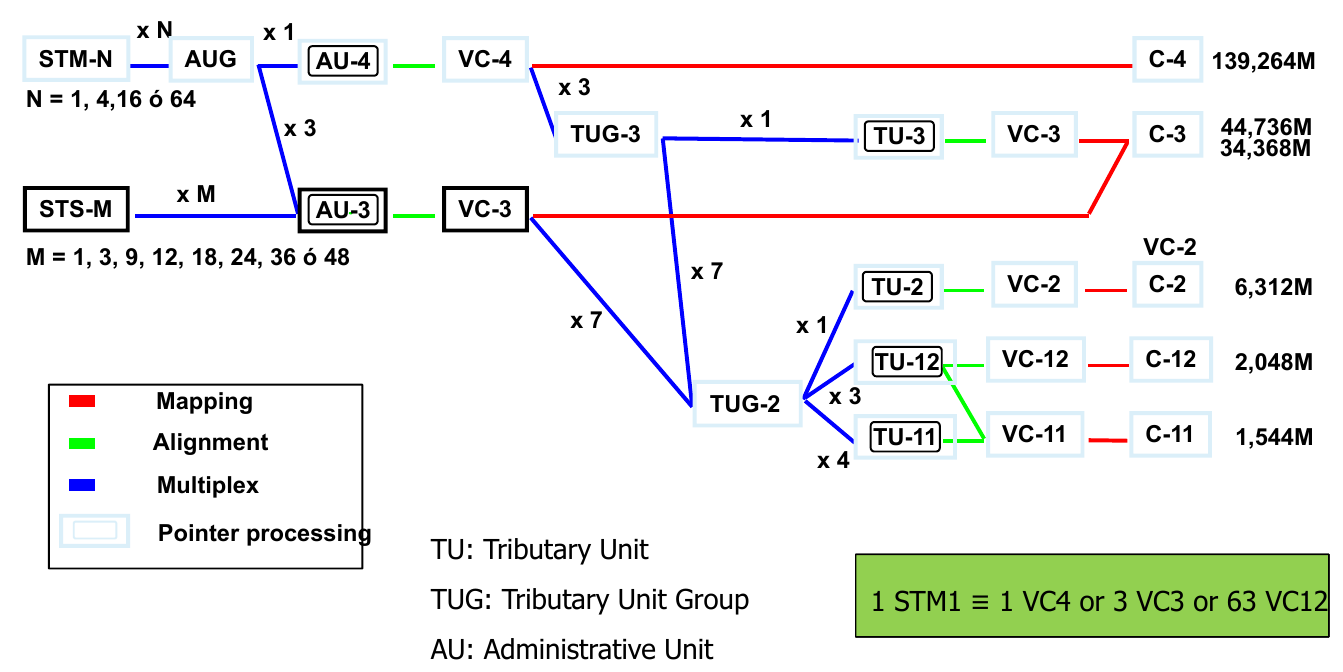
\includegraphics[
		width=12cm,
		%height=15cm
	]{images/Tema 3/SDH multiplex.png}
	\caption{
		\label{fig:unit3_STM1_multiplex}
		SDH multiplex
	}
\end{figure}

\subsection{Equipment}

Equipment includes:

\begin{itemize}
	\item {
		Regenerator

		\begin{figure}[H]
			\centering
			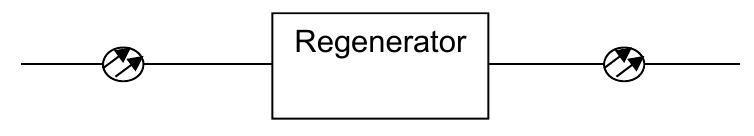
\includegraphics[
				width=7cm,
				%height=15cm
			]{images/Tema 3/Regenerator.png}
			\caption{
				\label{fig:unit3_regenerator}
				SDH regenerator
			}
		\end{figure}
	}
	\item {
		Terminal multiplexer (TM)

		\begin{figure}[H]
			\centering
			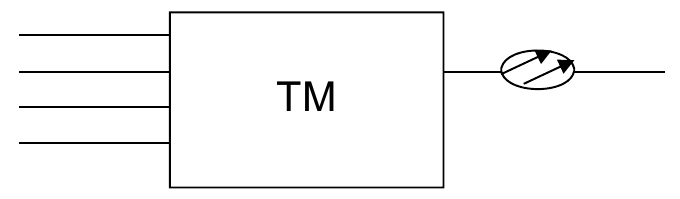
\includegraphics[
				width=5cm,
				%height=15cm
			]{images/Tema 3/TM.png}
			\caption{
				\label{fig:unit3_TM}
				SDH terminal multiplexer (TM)
			}
		\end{figure}
	}
	\item {
		Add and drop multiplexer (ADM)

		\begin{figure}[H]
			\centering
			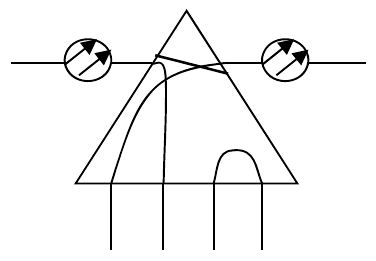
\includegraphics[
				width=4cm,
				%height=15cm
			]{images/Tema 3/ADM.png}
			\caption{
				\label{fig:unit3_ADM}
				SDH add and drop multiplexer (ADM)
			}
		\end{figure}
	}
	\item {
		Digital cross-connect (DXC)

		\begin{figure}[H]
			\centering
			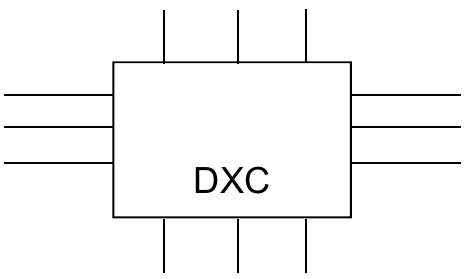
\includegraphics[
				width=4cm,
				%height=15cm
			]{images/Tema 3/DXC.png}
			\caption{
				\label{fig:unit3_DXC}
				SDH digital cross-connect (DXC)
			}
		\end{figure}
	}
\end{itemize}

\iffalse
Hardware protection
In hardware, protection techniques are used to avoid data loss due to failures in transmission equipment.
In SDH, five sections implement protection techniques:
- Tributary: It provides bandwidth to end user.
- Aggregate: It transmits and receives STM frames from one point to another.
- Controller and communication: It is responsible of NE communication and controlling.
- Cross connect: It is responsible of mapping tributary signals.
- Power supply: It provides a power supply to transmission equipment.
\fi

\subsection{Protection systems in optical networks}

\subsubsection{Introduction}

Protection is one of the two main strategies to guarantee quality of service on backbone networks:
\begin{itemize}
	\item Based on protection: They use preassigned capacity to replace transport entities when those fail.
	\item Based on restoration: They use rerouting. They require a management system.
\end{itemize}

Its implementation is carried out through management of common resources like connections and paths. There are several architectures for the implementation:
\begin{itemize}
	\item $1+1 \rightarrow$ There is a protection entity for each transport entity. Traffic is transmitted through both entities.
	\item $1:1 \rightarrow$ There is a protection entity for each transport entity. When protection entities is not being used, it can be used for low-priority traffic.
	\item $M:N \rightarrow$ There are $M$ protection entities for $N$ transport entities. It works in the same way as $1:1$ architecture.
\end{itemize}

When two nodes notice that the traffic going towards one direction has failed (unidirectional failure), the traffic can be switched to the protection entity in two modes:
\begin{itemize}
	\item Single-ended switching $\rightarrow$ Only the traffic going towards the affected direction is switched to the protection entity.
	\item Dual-ended switching $\rightarrow$ Traffic going towards any direction is switched to the protection entity.
\end{itemize}

\subsubsection{Path protection schemes}

One working path is replaced by one protection path.

\textbf{Multiplex Section-Lineal Protection (MS-LP)}
\begin{itemize}
	\item $1+1$ architecture.
	\item It has two different multiplexing physical paths.
\end{itemize}

\textbf{Multiplex Section-Shared Protection Ring (MS-SP Ring)}
\begin{itemize}
	\item $1:N$ architecture.
	\item Dual-ended switching.
	\item It spreads evenly work and protection capacity, half of VC’s are reserved for working paths and the other half is reserved for protection paths.
	\item If a link goes down, the two adjacent nodes use the switching protection, they deviate the traffic to the opposite direction.
	\item In case of failure at one point, the whole network can be regenerated.
\end{itemize}

\begin{figure}[H]
	\centering
	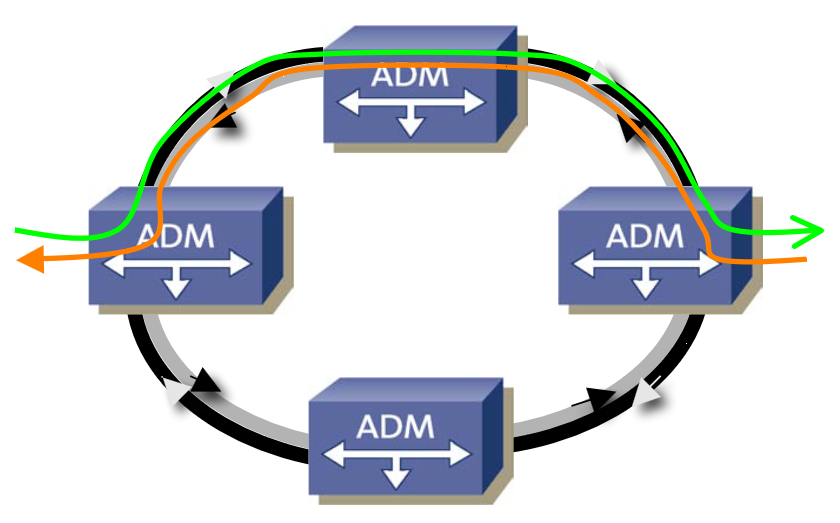
\includegraphics[
		width=7cm,
		%height=15cm
	]{images/Tema 3/ms_sp_ring_1.png}
	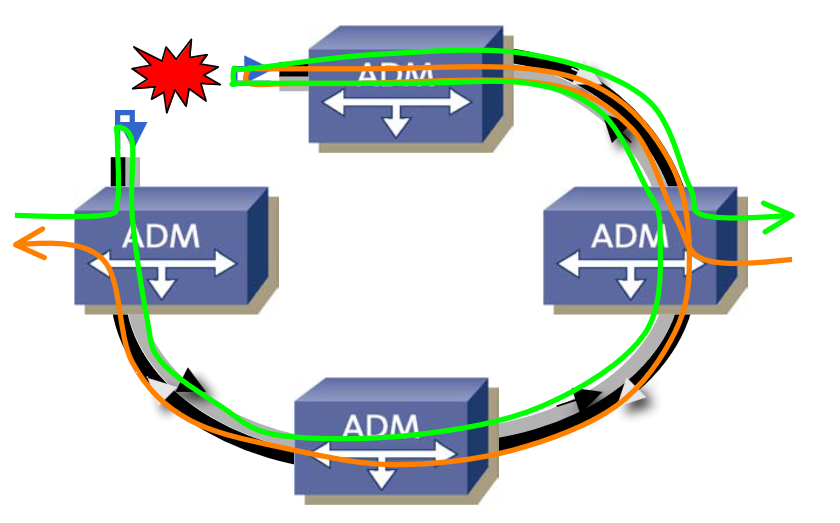
\includegraphics[
		width=7cm,
		%height=15cm
	]{images/Tema 3/ms_sp_ring_2.png}
	\caption{
		\label{fig:unit3_MS_SPRing}
		SDH MS-SP Ring
	}
\end{figure}

\textbf{Multiplex Section-Dedicated Protection Ring (MS-DP Ring)}

Similar to MS-SP Ring protection, but in a bidirectional connection, each sense takes a different path.

\begin{figure}[H]
	\centering
	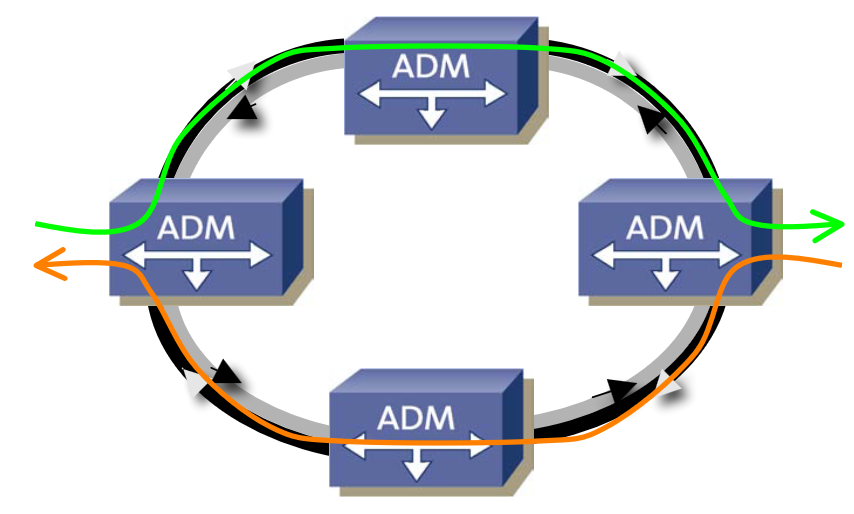
\includegraphics[
		width=7cm,
		%height=15cm
	]{images/Tema 3/ms_dp_ring_1.png}
	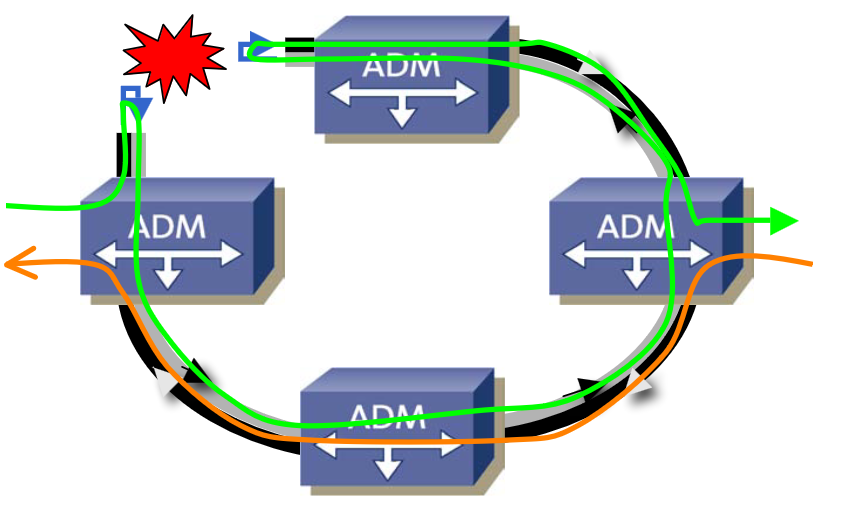
\includegraphics[
		width=7cm,
		%height=15cm
	]{images/Tema 3/ms_dp_ring_2.png}
	\caption{
		\label{fig:unit3_MS_DPRing}
		SDH MS-DP Ring
	}
\end{figure}

\textbf{HO-Trial protection}
\begin{itemize}
	\item $1:1$ architecture.
	\item Single-ended switching.
	\item It provides a dedicated end-to-end protection.
	\item It can be used in any physical topology (ring, mesh, etc.).
	\item The failure will be detected when it’s ending the Termination of higher-order path function.
\end{itemize}

\subsubsection{Sub-network connection protection schemes}

One working sub-network connection is replaced by one protection sub-network connection. It can be used at any physical topology.

\textbf{Subnetwork Connection Protection ring (SNCP)}
\begin{itemize}
	\item $1+1$ architecture.
	\item Single-ended protection.
	\item Traffic is transmitted through working sub-network connection and protection sub-network connection at the same time.
	\item A switch is used to select the sub-network connection.
\end{itemize}

\begin{figure}[H]
	\centering
	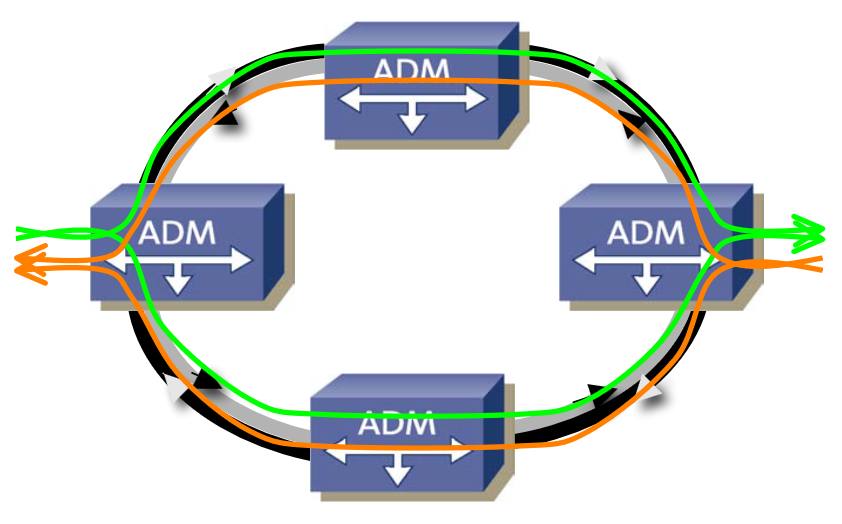
\includegraphics[
		width=7cm,
		%height=15cm
	]{images/Tema 3/sncp.png}
	\caption{
		\label{fig:unit3_sncp}
		SDH SNCP
	}
\end{figure}

\textbf{Drop\&Continue protection}
\begin{itemize}
	\item It is used at ring junctions to add connections between them.
	\item It improves the availability of sub-networks. For example, it supports two failures when they have happened in different things.
\end{itemize}

\section{(Dense) Wavelength Division Multiplexing ((D)WDM)}

\subsection{Introduction}

The all-optical networks are very young (since 2000):

\begin{itemize}
	\item {
		Until 2000, almost optical networks:
		\begin{itemize}
			\item Only fiber.
			\item One wavelength, usually 1310 nm (optimized) in singlemode fibers.
			\item Optical-electrical interfaces are inefficient.
		\end{itemize}
	}
	\item In 80, 50 Mbps (ODL-50 devices).
	\item Proprietary designs appeared. All disappeared with SONET/SDH.
	\item Limit per fiber is 40 Gbps (10 Gbps in 90’s).
	\item In 90’s, large bandwidth demands. Several fibers are put together.
\end{itemize}

New technologies such as WDM (Wavelength Division Multiplexing) and Dense WDM came up:

\begin{itemize}
	\item A single fiber carries several wavelengths. Example: 40 wavelengths per fiber, each with 40 Gbps gives 1.6 Tbps per fiber.
	\item Between 8 - 32 wavelengths: Coarse WDM
	\item More than 40: DWDM
\end{itemize}

\begin{figure}[H]
	\centering
	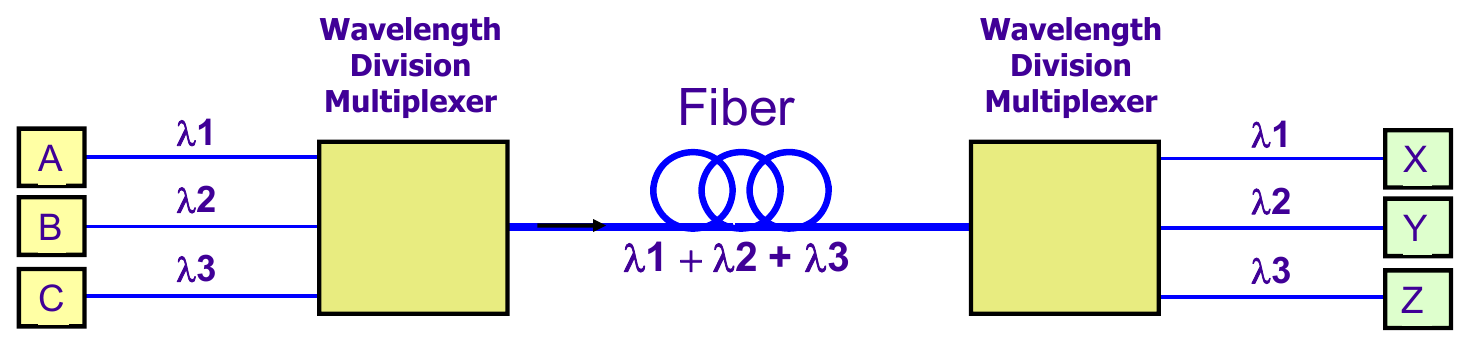
\includegraphics[
		width=12cm,
		%height=15cm
	]{images/Tema 3/(D)WDM.png}
	\caption{
		\label{fig:unit3_DWDM}
		(D)WDM sheme
	}
\end{figure}

It is highly likely that in near future we will have FttPC (Fiber to the PC).

Advantages:

\begin{itemize}
	\item Large capacity per fiber
	\item {
		Scales easily:
		\begin{itemize}
			\item No new fibers are needed, only add new wavelengths.
			\item Incremental cost per extra channel is low.
			\item No too much changes in the hardware.
		\end{itemize}
	}
	\item The fiber span is much larger with DWDM than TDM (SONET/SDH). Chromatic dispersion and polarization in TDM
\end{itemize}

Disadvantages:

\begin{itemize}
	\item Very expensive for few channels. Fixed costs such as the mux/demux, transponders and other components.
	\item Introduces a new parameter in the design and management: the wavelength.
	\item SONET/SDH networks are not well prepared for DWDM.
	\item Monitoring DWDM signals still needs research.
\end{itemize}

\subsection{CWDM Advantages}

CWDM is cheaper than DWDM, about 30\%. That’s because:

\begin{itemize}
	\item Cheaper lasers since less precision and control is required.
	\item Passive components such as multiplexers can be obtained at low cost.
	\item CWDM components need less physical space in PCBs, which implieas a lower cost.
\end{itemize}

\subsection{SXG-PON}

PON (Pasive Optical Network). Provide FTTH services.

\begin{tabular}{|l|l|l|l|l|}
	\hline
						& G-PON	& XG-PON	& SXG-PON	& NG-PON \\
	\hline
	Upstream (Gbps)		& 1,5	& 2,5		& 10		& 40 \\
	\hline
	Downstream (Gbps)	& 2,5	& 10		& 10		& 40 \\
	\hline
						& Gigabit			& 10 Gbit	& Symmetric XG	& Next generation \\
	\hline
\end{tabular}

\subsection{Applications}

Main applications:

\begin{itemize}
	\item Metropolitan Area Networks. Up to FttPC.
	\item CATV
\end{itemize}

Supports:

\begin{itemize}
	\item IP
	\item SDH/SONET
	\item ATM
	\item Frame-Relay
	\item Ethernet
	\item Multi-protocol Label System (MPLS) and its adaptation M$\lambda$LS.
\end{itemize}



\end{document}
